\documentclass[14pt,aspectratio=169]{beamer}

\usepackage{pgfpages}
\usepackage{fancyvrb}

\usepackage{tikz}
\usepackage{pgfplots}

\usepackage{minted}
\usemintedstyle{tango}

\usepackage{graphicx}

\usetheme{auriga}
\usecolortheme{auriga}

\setbeamercolor{background canvas}{bg=lightgray}

% define some colors for a consistent theme across slides
\definecolor{red}{RGB}{181, 23, 0}
\definecolor{blue}{RGB}{0, 118, 186}
\definecolor{gray}{RGB}{146, 146, 146}

\title{Web Development: \\ Creating Tables and Forms}

\author{{\bf Gregory M. Kapfhammer}}

\institute[shortinst]{{\bf Department of Computer Science, Allegheny College}}

\begin{document}

{
  \setbeamercolor{page number in head/foot}{fg=background canvas.bg}
  \begin{frame}
    \titlepage
  \end{frame}
}

% Slide
%
\begin{frame}{Technical Question}
  %
  \hspace*{.25in}
  %
  \vspace*{.1in}
  %
  \begin{minipage}{4.5in}
  %
  \begin{center}
    %
    {\large How can I follow industry best practices to use both HTML and CSS to
    implement tables that display formatted content and forms that receive and
  verify user input?}
    %
  \end{center}
  %
  \end{minipage}
  %
  \vspace{2ex}
  %
  \begin{center}
    %
    \small Let's learn how to combine CSS and HTML to create tables and forms!\\
    \small We focused on tables last week and now forms this week!\\
    \small Since web development in cumulative, please review all previous content!\\
    %
  \end{center}
  %
\end{frame}

% Slide
%
\begin{frame}{User Input with HTML5 Forms}
  %
  \begin{itemize}
    %
    \item Before HTML5, user input and form customization was limited; now
      multiple tags, CSS styling options, and services exist. Static sites
      present additional challenges!
      %
      \vspace*{-.15in}
      %
    \item Some examples of form components in HTML:
      %
      \begin{itemize}
        %
        \item Lists, radio buttons, and checkboxes
          %
        \item Form submission buttons and controls
          %
        \item Controls for input of text and file uploads
          %
      \end{itemize}
      %
      \vspace*{-.2in}
      %
    \item What type of content is best requested in a form?
      %
      \vspace*{-.2in}
      %
    \item What are not the most appropriate uses of a form?
      %
      \vspace*{-.2in}
      %
    \item What are the challenges associated with creating a form?
      %
  \end{itemize}
  %
\end{frame}

% Slide
%
\begin{frame}{The Lifecycle of Form Interaction}
  %
  \begin{itemize}
    %
    \item Does the web server provide a database for storage?
      %
      \vspace*{-.2in}
      %
    \item Does the web client support JavaScript or form validation?
      %
      \vspace*{-.2in}
      %
    \item The lifecycle of form creation and interaction:
      %
      \begin{itemize}
        %
        \item Developer creates a form and publishes to a web page
          %
        \item Developer connects the form to a data storage endpoint
          %
        \item Person views the form and submits the required content
          %
        \item The web client validates the form's current content
          %
        \item The web client transmits form content to the server
          %
      \end{itemize}
      %
      \vspace*{-.25in}
      %
    \item What are the challenges associated with creating a form?
      %
      \vspace*{-.25in}
      %
    \item What are the trade-offs associated with HTML forms?
      %
  \end{itemize}
  %
\end{frame}

% Slide
%
\begin{frame}{Using Formspree in Static Sites}
  %
  \begin{figure}
    \centering
    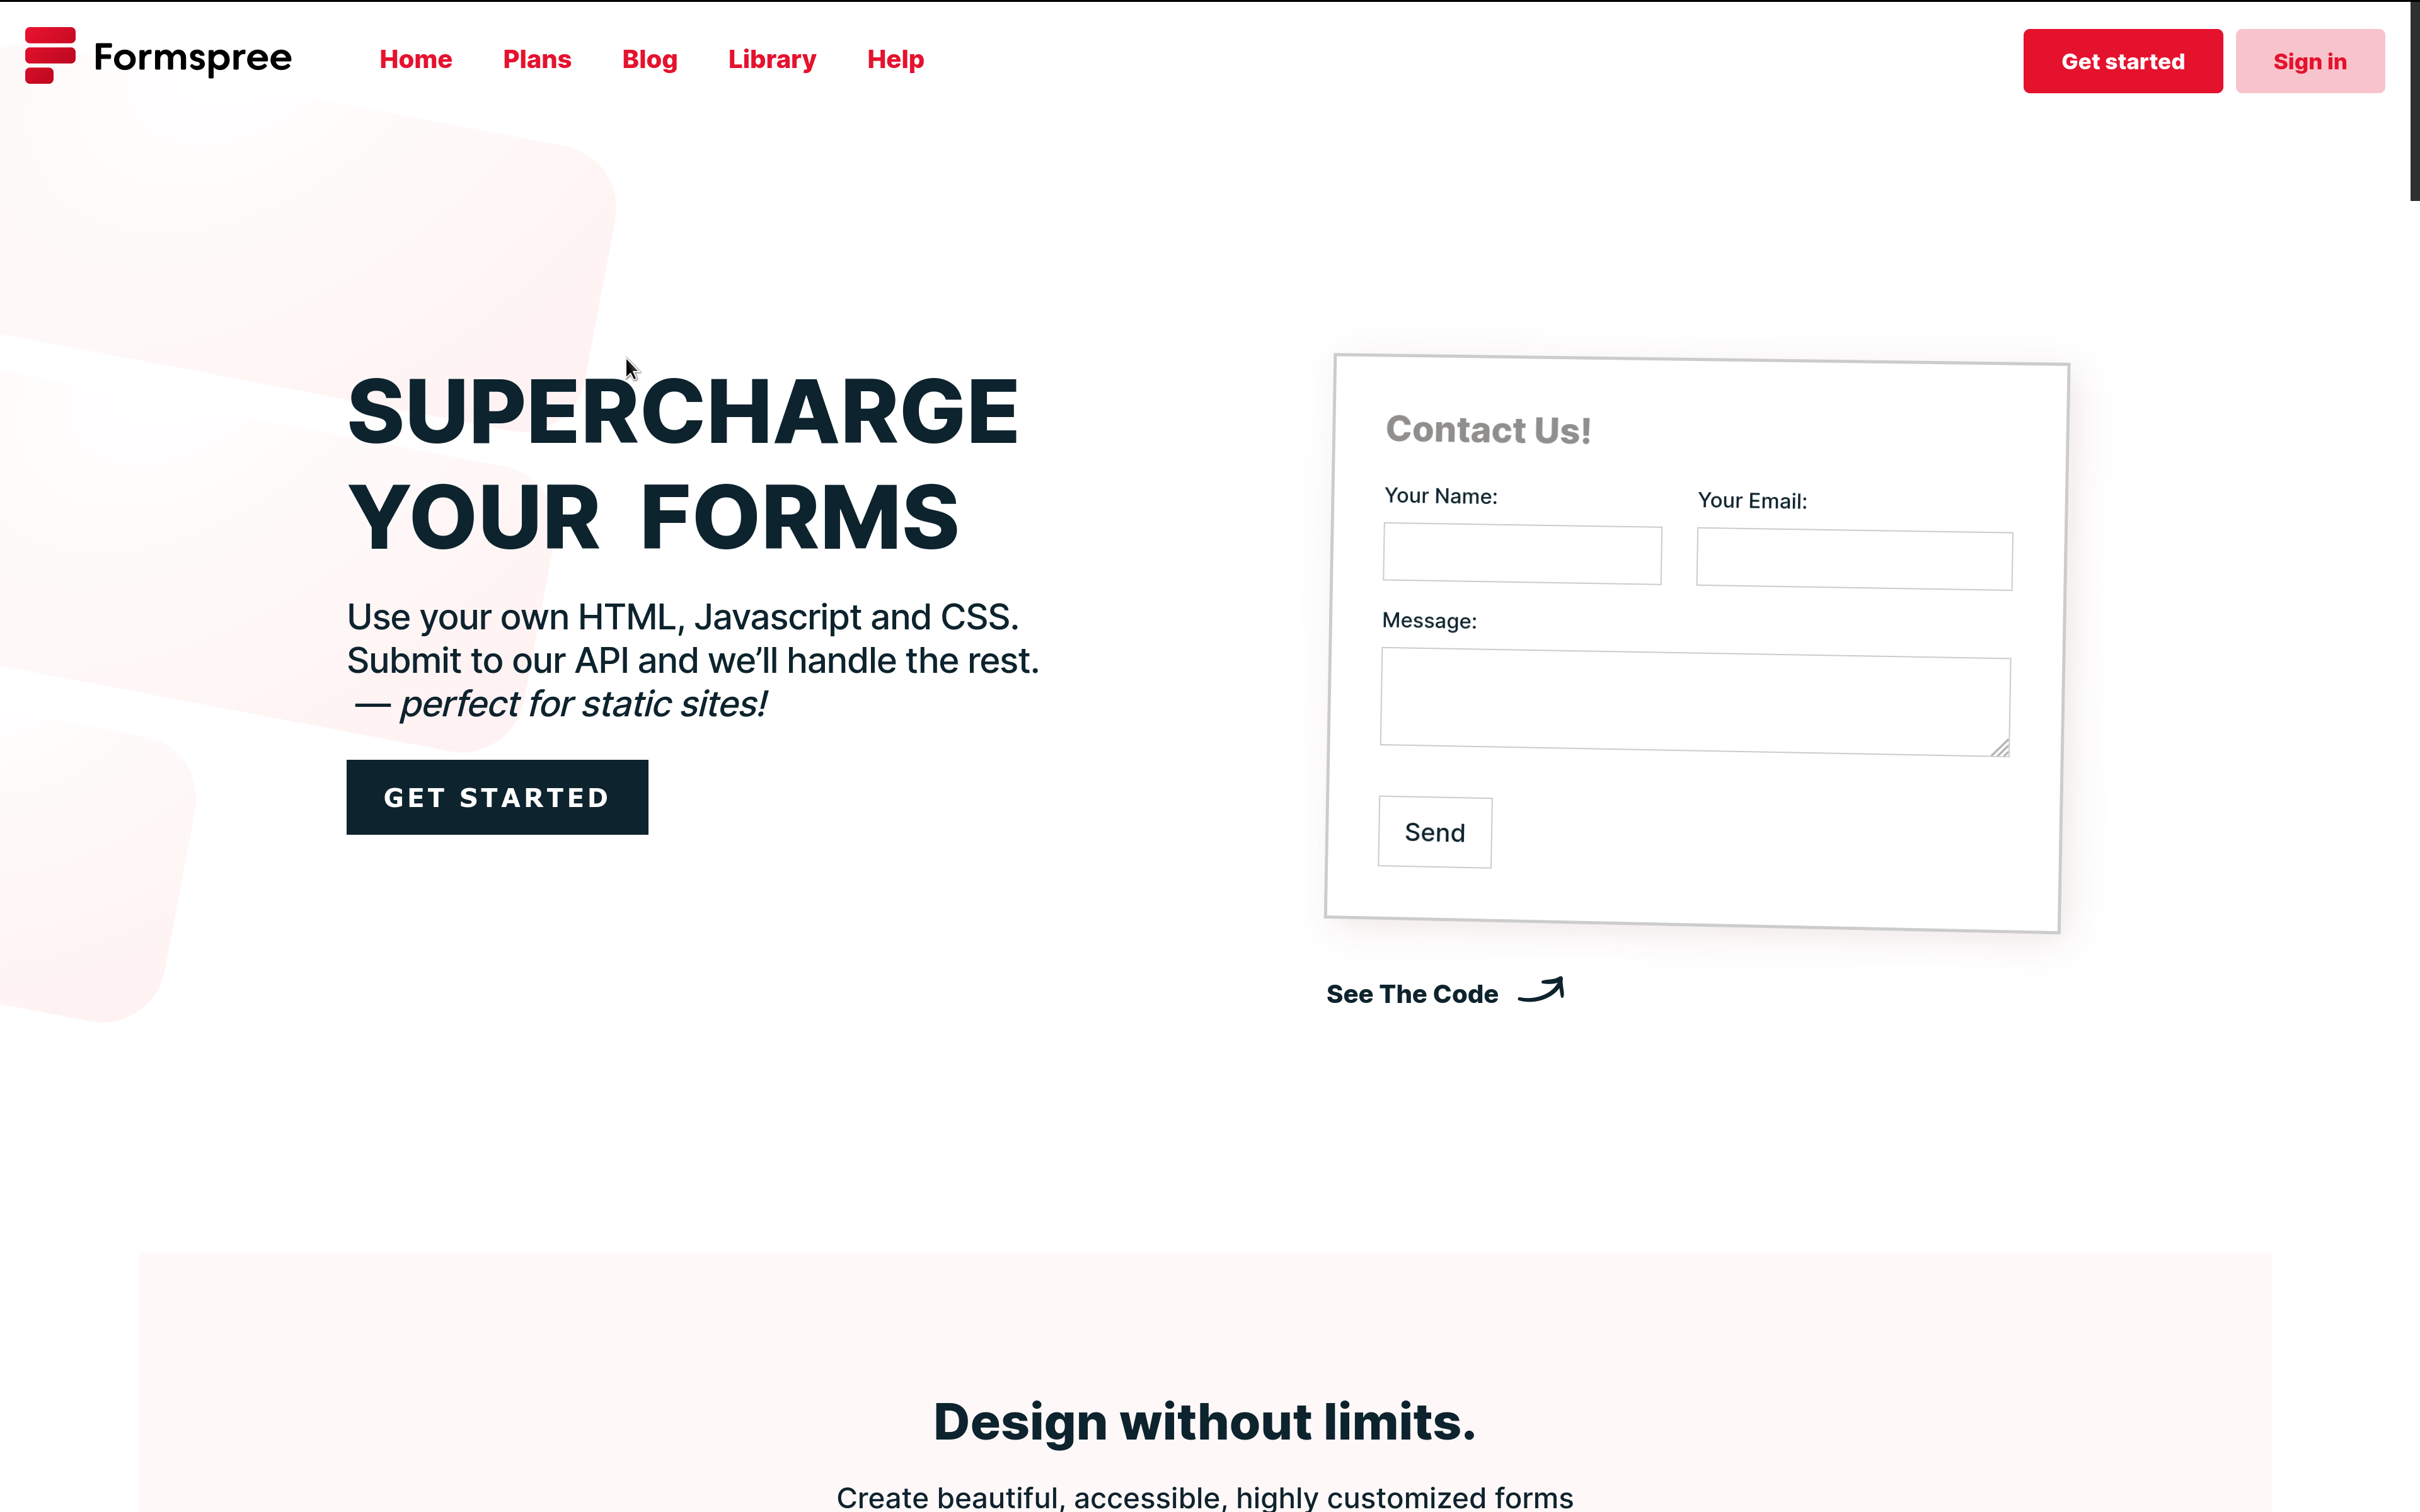
\includegraphics[scale=.08]{images/formspree.png}
    \caption{The figure's caption}
  \end{figure}
  %
\end{frame}

% Slide
%
\begin{frame}{Using Netlify Forms in Static Sites}
  %
  \begin{figure}
    \centering
    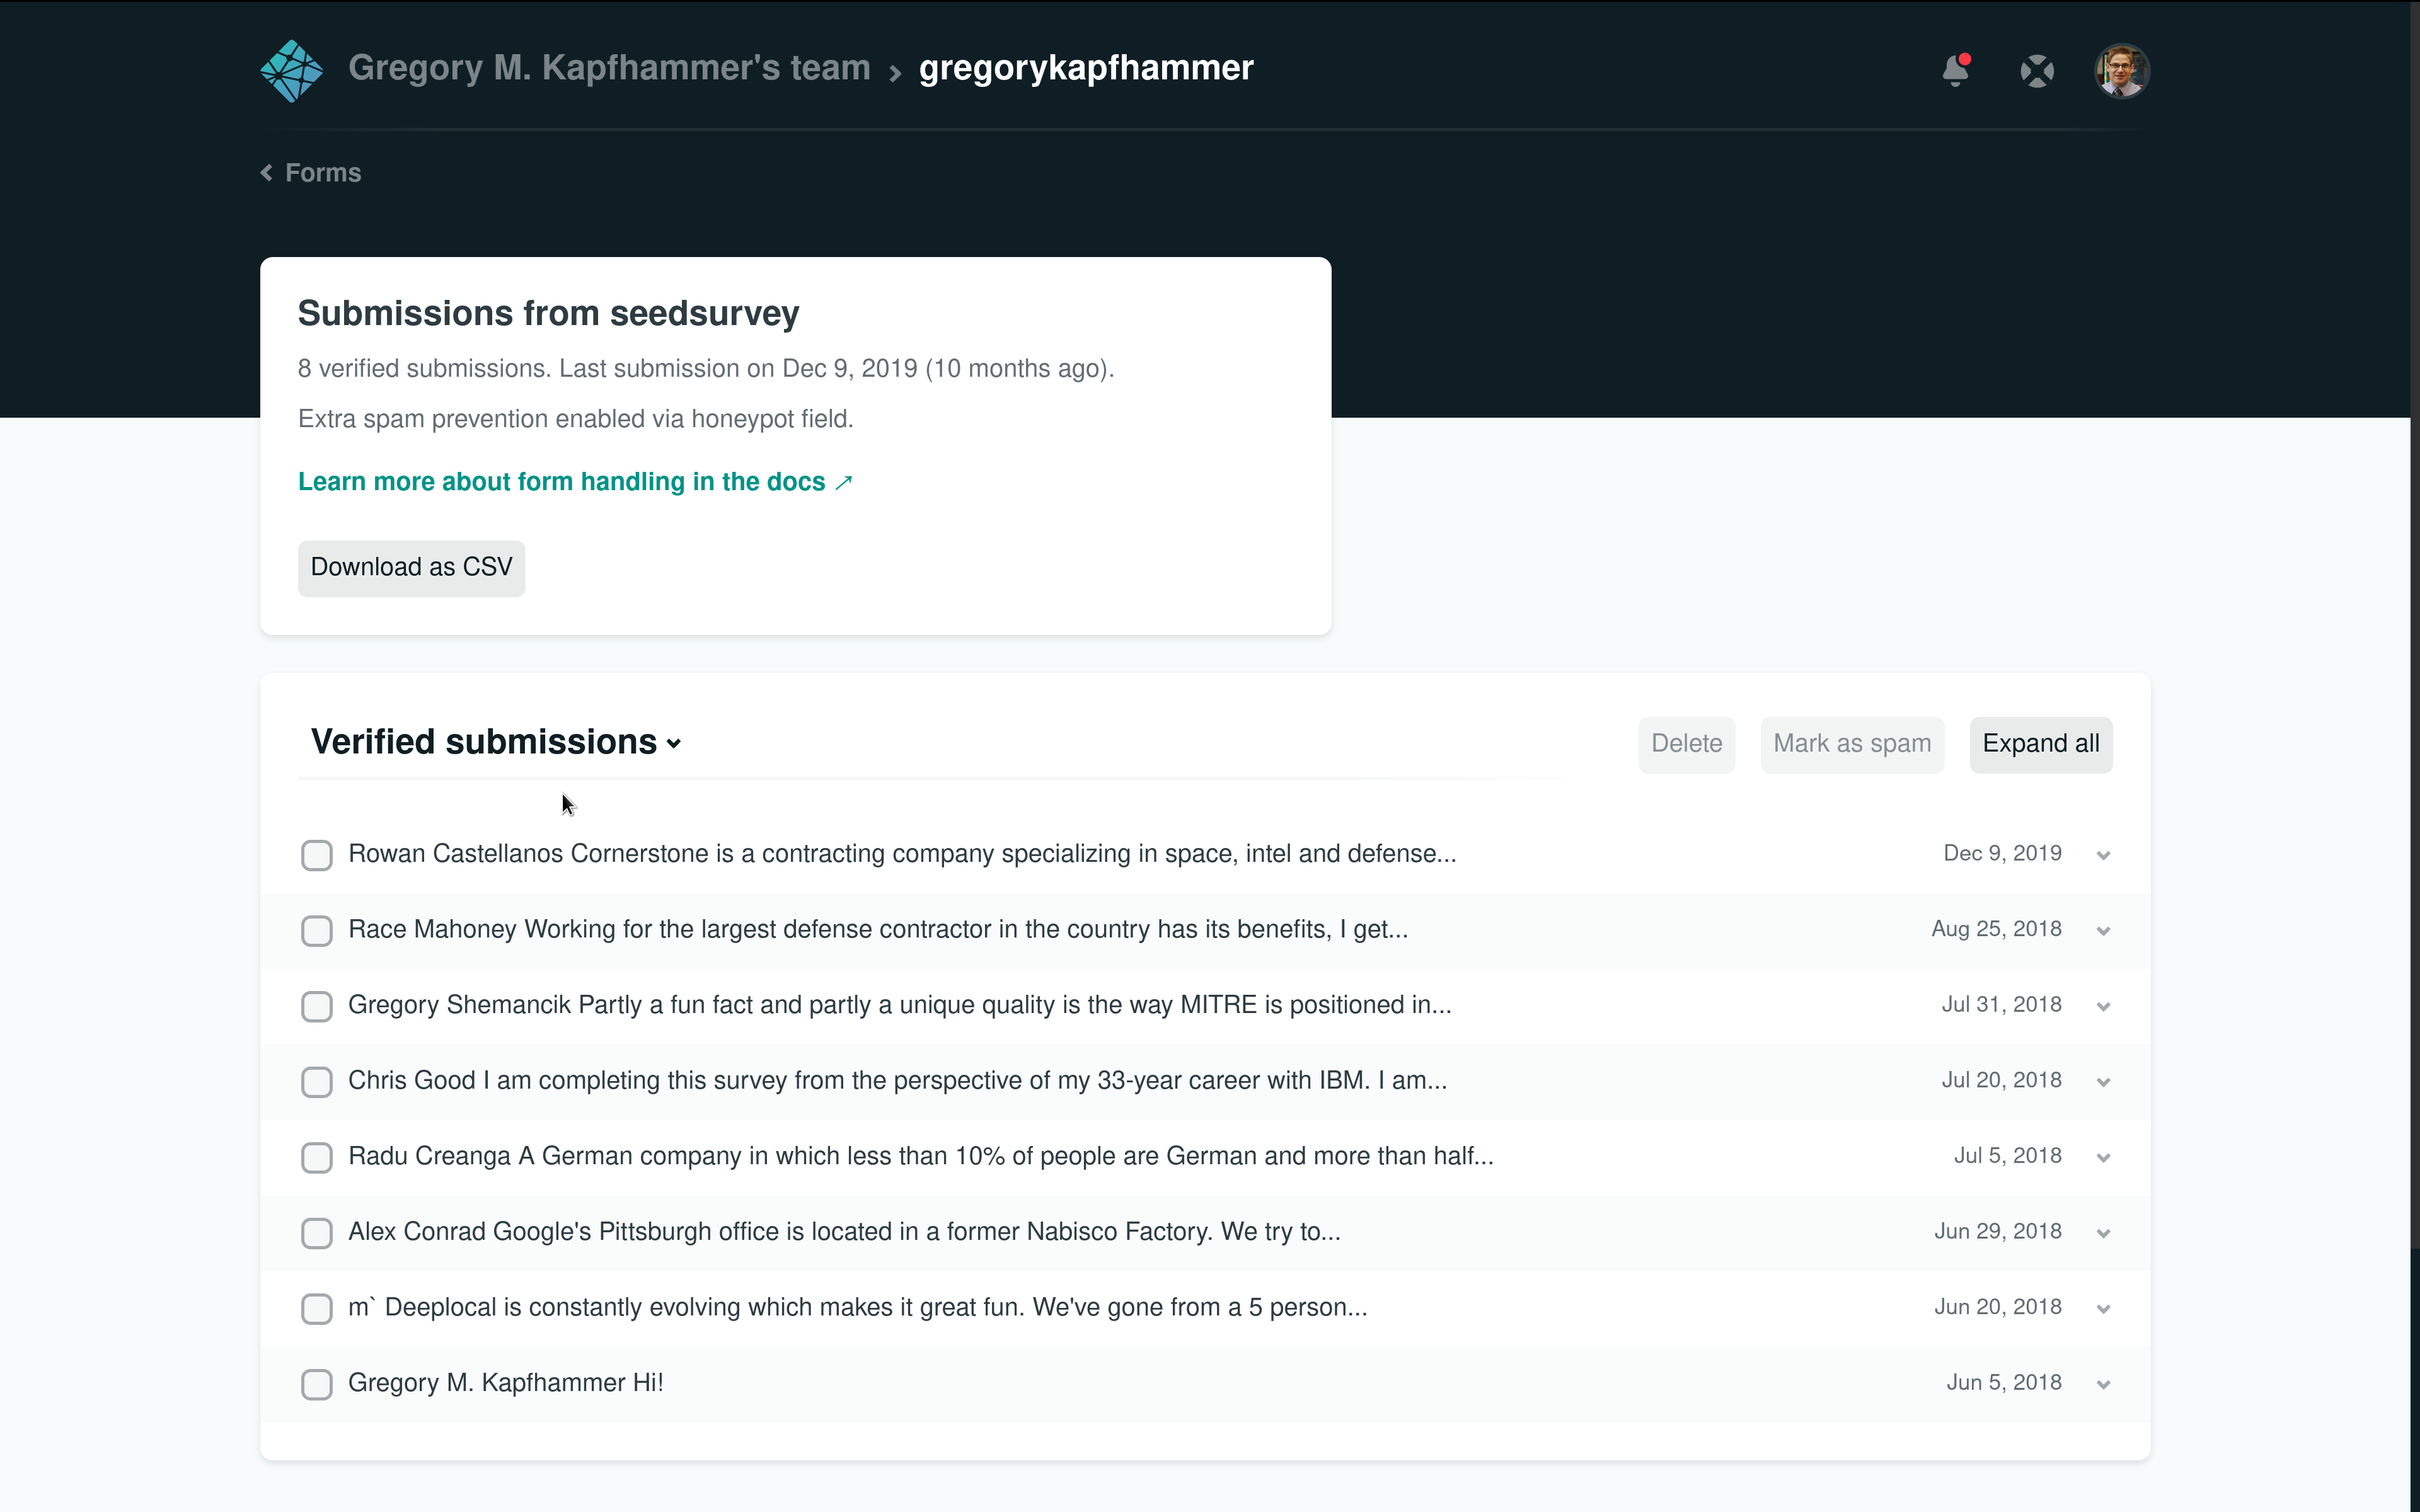
\includegraphics[scale=.08]{images/netlifyforms.png}
    \caption{The figure's caption}
  \end{figure}
  %
\end{frame}

% Slide
%
\begin{frame}[fragile]
  \frametitle{Programming HTML Forms Using Formspree}
  \normalsize
  \begin{minipage}{6in}
    \vspace*{.1in}
    \begin{minted}[mathescape, numbersep=5pt, fontsize=\large]{html}
    <form
      action="https://formspree.io/
              gkapfham@
              allegheny.edu"
      method="POST">
      Share your Views!
      <input type="submit"
      value="Submit">
    </form>
    \end{minted}
  \end{minipage}
  %
\end{frame}

% Slide
%
\begin{frame}[fragile]
  \frametitle{Creating Labels and Form Controls}
  \normalsize
  \begin{minipage}{6in}
    \vspace*{.1in}
    \begin{minted}[mathescape, numbersep=5pt, fontsize=\large]{html}
<label>Name</label>
<input type="text" name="name">
<label>Email</label>
<input type="email" name="_replyto">
    \end{minted}
  \end{minipage}
  \vspace*{.05in}
  \begin{center}
    %
    \noindent This content would exist inside of a {\tt <form>} \\
    %
    \noindent Forms can contain labels for content and form controls \\
    %
    \noindent CSS from Bootstrap can control form control layout \\
    %
  \end{center}
  %
\end{frame}

% Slide
%
\begin{frame}[fragile]
  \frametitle{Creating Dropdown Lists in Forms}
  \normalsize
  \begin{minipage}{6in}
    \vspace*{.1in}
    \begin{minted}[mathescape, numbersep=5pt, fontsize=\large]{html}
<label>What is your preferred city?
</label>
<input type="text" name="city"
  list="cities"/>
<datalist id="cities">
  <option>Calcutta</option>
  <option>Calgary</option>
  <option>London</option>
</datalist>
    \end{minted}
  \end{minipage}
  \vspace*{.05in}
  \begin{center}
    %
    % \noindent This content would exist inside of a {\tt <form>} \\
    %
  \end{center}
  %
\end{frame}

% Slide
%
\begin{frame}[fragile]
  \frametitle{Creating Radio Buttons in Forms}
  \normalsize
  \begin{minipage}{6in}
    \vspace*{.1in}
    \begin{minted}[mathescape, numbersep=5pt, fontsize=\large]{html}
<label>What is your favorite continent?
</label>
<input type="radio"
  name="continent" value="1">
  North America
<input type="radio"
  name="continent" value="2">
  South America
    \end{minted}
  \end{minipage}
  \vspace*{.05in}
  \begin{center}
    %
    % \noindent This content would exist inside of a {\tt <form>} \\
    %
  \end{center}
  %
\end{frame}

% Slide
%
\begin{frame}[fragile]
  \frametitle{Creating Checkboxes in Forms}
  \normalsize
  \begin{minipage}{6in}
    \vspace*{.1in}
    \begin{minted}[mathescape, numbersep=5pt, fontsize=\large]{html}
<label>What country will you visit?
</label>
<input type="checkbox"
  name="country" value="canada">Canada
<input type="checkbox"
  name="country" value="france">France
    \end{minted}
  \end{minipage}
  \vspace*{.05in}
  \begin{center}
    %
    \noindent What convention do we follow for picking form controls? \\
    %
    \noindent How do ensure correctness of layout and user interaction? \\
    %
  \end{center}
  %
\end{frame}

% Slide
%
\begin{frame}[fragile]
  \frametitle{Creating Text Areas in Forms}
  \normalsize
  \begin{minipage}{6in}
    \vspace*{.1in}
    \begin{minted}[mathescape, numbersep=5pt, fontsize=\large]{html}
<label>What is your travel story?
</label>
<textarea rows="3"
  cols="80"
  name="story">
  Share your travel story
  </textarea>
    \end{minted}
  \end{minipage}
  \vspace*{.05in}
  \begin{center}
    %
    \noindent How do we ensure that forms do not submit malicious content? \\
    %
    \noindent How do we ensure that forms provide a good user experience? \\
    %
  \end{center}
  %
\end{frame}

% Slide
%
\begin{frame}[fragile]
  \frametitle{Using Bootstrap to Layout Forms}
  \normalsize
  \begin{minipage}{6in}
    \vspace*{.1in}
    \begin{minted}[mathescape, numbersep=5pt, fontsize=\normalsize]{html}
  <div class="form-group">
    <label for="name">Name</label>
    <div class="row">
      <div class="col">
        <input type="text"
          class="form-control"
          name="name" id="name"
          placeholder="Your name" required>
      </div>
    </div>
  </div>
    \end{minted}
  \end{minipage}
  %
\end{frame}

% Slide
%
\begin{frame}[fragile]
  \frametitle{Defining Placeholders for Form Inputs}
  \normalsize
  \begin{minipage}{6in}
    \vspace*{.1in}
    \begin{minted}[mathescape, numbersep=5pt, fontsize=\normalsize]{html}
  <div class="form-group">
    <label for="reply_to">Email</label>
    <div class="row">
      <div class="col">
        <input type="email"
           class="form-control"
           name="reply_to" id="reply_to"
           placeholder="user.name@example.com"
           required>
      </div>
    </div>
  </div>
    \end{minted}
  \end{minipage}
  %
\end{frame}

% Slide
%
\begin{frame}[fragile]
  \frametitle{Specifying Data Types for Form Inputs}
  \normalsize
  \begin{minipage}{6in}
    \vspace*{.1in}
    \begin{minted}[mathescape, numbersep=5pt, fontsize=\normalsize]{html}
  <div class="form-group">
    <label for="web_site">Web Site</label>
    <div class="row">
      <div class="col">
        <input type="url"
           class="form-control"
           name="web_site" id="web_site"
           placeholder="Your web site"
           required>
      </div>
    </div>
  </div>
    \end{minted}
  \end{minipage}
  %
\end{frame}

% Slide
%
\begin{frame}[fragile]
  \frametitle{Specifying Data Types for Form Inputs}
  \normalsize
  \begin{minipage}{6in}
    \vspace*{.1in}
    \begin{minted}[mathescape, numbersep=5pt, fontsize=\normalsize]{html}
  <div class="form-group">
    <label for="time">How many minutes
       did it take to complete survey?</label>
    <div class="row">
      <div class="col">
        <input type="number"
           class="form-control"
           name="time" id="time"
           min=1 step=1>
      </div>
    </div>
  </div>
    \end{minted}
  \end{minipage}
  %
\end{frame}

\end{document}
